%\documentclass[12pt,a4paper]{article}
\documentclass[12pt,a4paper]{IEEEtran}
\usepackage[margin=0.65in]{geometry}
\usepackage[affil-it]{authblk}
\usepackage{graphicx}
\usepackage[table,xcdraw]{xcolor}
\usepackage{caption}
\usepackage{subcaption}
\usepackage{float}
\usepackage{hyperref}
\usepackage{relsize}
\usepackage{amsmath}
{
	%	\theoremstyle{plain}
	\newtheorem{assumption}{Assumption}
}
\usepackage[most]{tcolorbox}
\tcbset{textmarker/.style={%
		enhanced,
		parbox=false,boxrule=0mm,boxsep=0mm,arc=0mm,
		outer arc=0mm,left=6mm,right=3mm,top=7pt,bottom=7pt,
		toptitle=1mm,bottomtitle=1mm}}

\newtcolorbox{importantBox}{textmarker,
	borderline west={6pt}{0pt}{red},
	colback=red!10!white}

\newcommand{\important}[1]{\begin{importantBox} \textbf{Important:} #1 \end{importantBox}}
\newcommand{\magn}[1]{\Vert{#1}\Vert}
\newcommand{\card}[1]{\vert{#1}\vert}

\title{Perimeter Compression in self-healing swarms}
\author[1,*]{Neil Eliot}
\author[2]{David Kendall}
\author[2]{Michael Brockway}
\affil[1] {Northumbria University, Faculty of Engineering and Environment, Department of Computer and Information Sciences}
\affil[2] {Hexham University, Faculty of Computer Science}
\affil[*] {Corresponding author: Dr Neil Eliot, neil.eliot@northumbria.ac.uk}
\date{\today}


\begin{document}
\maketitle

\begin{abstract}
Perimeter Compression is a technique where by a void reducing effect can be added to a basic swarming algorithm. The affect is dependant upon perimeter identification and is controlled by applying two weighting factors to the existing swarming formulae. One to the cohesion calculation and the other to the repulsion calculation.
\end{abstract}

\section{Introduction}
When cohesion and repulsion field effects are used to create a swarming effect, the stable structures that develop are limited to either straight edges or partial lattices \cite{eliot2017methods}. The maintenance of a well-structured swarm is crucial to effective deployment, including reconnaissance or artificial pollination, where `blind spots' are best  eliminated \cite{elamvazhuthi2015optimal}, and containment, where the swarm is used to surround an object or region \cite{cao2012distributed}. Over time swarms form regular shapes~\cite{RAZ:13} and perimeters form of partial lattices may contain so-called \textit{anomalies}, such as concave `dents' or convex `peaks'. These anomalies contribute to the disruption of an otherwise well-structured swarm. The key, therefore, is to ensure that these \textit{anomalies} are dynamically removed from a swarm.\\
Perimeter compression is a technique that creates a `pull' effect between perimeter agents. It is dependant upon perimeter agent identification as discussed by Eliot et. al. in \cite{eliot2017methods, eliot2018metric, eliot2019void} and shown in Section~\ref{perimeterDetection}.\\
The aim of the algorithm is to reduce the spacing between perimeter-based agents by reducing the repulsion field and increasing the cohesion affect on perimeter agents. Figure \ref{fig:stableswarm}) shows an agent and it fields. $S_b$ is the sensor field. $O_b$ is the obstacle field. $C_b$ is the cohesion field and $R_b$ is the repulsion field. The implementation involves introducing two controlling weights; $p_c$ (Perimeter Compression Cohesion) which increases the cohesion vector ($k_c\rightarrow p_ck_c$) and $p_r$ (Perimeter Compression Repulsion) which reduces the size of the repulsion field ($k_r\rightarrow p_rk_r$) of the perimeter-based agents.
\begin{assumption}
	$p_c >= 1$
\end{assumption}
\begin{assumption}
	$p_r <= 1$
\end{assumption}
\begin{figure}[H]
	\centering
	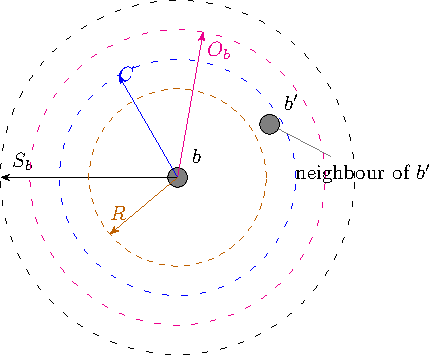
\includegraphics[width=0.8\linewidth]{figures/stableswarm}
	\caption[Agent Fields]{Agent Fields}
	\label{fig:stableswarm}
\end{figure}

\section{Related work}

As far back as 1987 swarm theory has adopted the use of potential fields to coordinate agents~\cite{REY:87} and this has continued since then in an attempt to improve the structure of a swarm, coordinate obstacles, and  improve navigation~\cite{BAFVM:06,BAF:06,BFV:07,BM:09,eliot2018metric,VG:05,HC:09,SW:03,Son2017}. A prototype framework for self-healing swarms was developed by Dai et al., which considered how to manage agent failure in hostile environments \cite{DHMRZ:06}. This was similar to work by Vassev and Hinchey, who modelled swarm movement using the ASSL (Autonomic System Specification Language) \cite{VH:09}. This technique was employed by NASA (US National Aeronautics and Space Administration) for use in asteroid belt exploration as part of their ANTS (Autonomous Nano Technology Swarm) project. However, this work is focused towards failure of an agent's internal systems, rather than on the removal of anomalies in a swarm distribution. 

In the context of swarm structure maintenance, Roach et al. focussed on the effects of sensor failure, and the impact that has on agent distribution \cite{RMT:15}. Lee and Chong identified the issue of concave edges within swarms in an attempt to create regular lattice formations \cite{GN:08}, and the main focus of their work is the dynamic restructuring of inter-agent formations. Ismail and Timmis demonstrated the use of \textit{bio-inspired} healing using \textit{granuloma formation}, a biological method for encapsulating an antigen \cite{IT:10}. They have also considered the effect that failed agents can have on a swarm when traversing a terrain \cite{TIBW:16}. 

This void reduction effect is an extension of the work presented by Eliot et al. \cite{eliot2019void}, Ismail and Timmis \cite{IT:10,TIBW:16}, and also builds on the work of Lee and Chong on concave edge identification \cite{GN:08}, and on the work of McLurkin and Demaine on the detection of perimeter types \cite{mclurkin2009}. However, perimeter type identification requires a communications infrastructure. The technique employed in this paper does not explicitly require the identification of the perimeter type as it would limit the size of the swarm\cite{eliot2019void,GN:08} and is therefore a reduced algorithm to identify any perimeter.

\section{Basic swarming model}\label{basicModel}
In the Original work by Eliot et. al. the resultant vector of an agent was calculated using Equation~\ref{eq:resultantVector1a}. Where $k_c,k_r,k_d,k_o$ are weighting factors for the summed vectors associated with each interaction. 

\begin{equation}\label{eq:resultantVector1a}
	v(b) = k_cv_c(b) + k_rv_r(b) + k_dv_d(b) + k_ov_o(b)
\end{equation}

In this paper we will only be considering the cohesion and repulsion components of the equation to create the new compression effect. (Eq.~\ref{eq:resultantVector2a}).

\begin{equation}\label{eq:resultantVector2a}
v(b) = k_cv_c(b) + k_rv_r(b)
\end{equation}

\subsection{Repulsion}\label{repulsion:neighbours}
The repulsion component of an agent's movement is calculated from interaction with its neighbours $n_r(b)$ (Eq.~\ref{eq:repulsion1a}) in a swarm ($\mathcal{S}$) that are within the agent's ($b$) repulsion field ($R_b$).

\begin{equation}\label{eq:repulsion1a}
n_r(b) = \{b' \in \mathcal{S} : b \neq b' \land \lVert\vec{b b'}\rVert \leq R_b)\}
\end{equation}

The repulsion is then calculated as the average of all the vectors created by the agent ($b$) to the neighbours ($b'$) (Eg.~\ref{eq:repulsion2a}) and its proximity ($\lVert\vec{bb'}\rVert - R_b$).

\begin{equation}\label{eq:repulsion2a}
v_r(b) = \frac{1}{\lvert n_r(b)\rvert}\sum_{b' \in n_r(b)} \left(\lVert\vec{b b'}\rVert - R_b \, \right)\widehat{bb'}
\end{equation}

\subsection{Cohesion}\label{cohesion}
The cohesion component of an agent is calculated in a similar way to the repulsion in that it is dependent upon the proximity of neighbours. Where $n_c(b)$ is the set of neighbour agents for $b$ (Eq. \ref{eq:cohesion1}). The inclusion of an agent from a swarm ($S$) in by the agent's cohesion field ($C_b$).

\begin{equation}\label{eq:cohesion1}
n_c(b) = \{b' \in S~:~b' \neq b \land\magn{bb'} <= C_b\}
\end{equation}

The affect of an agent being within this set is that it will generate a vector that should `encourage' agents to maintain their proximity. i.e. generate a cohesive swarm. The general weighted ($k_c$) formula for agents to maintain their proximity is to direct their motion towards the central point of all neighbouring agents as shown in Equation~\ref{eq:cohesion2}. This formula includes the $k_c$ quotient that allows the cohesion effect to be `balanced' with respect to other vector influences as described in ~\cite{eliot2017methods,eliot2018metric,eliot2019void} 

\begin{equation}\label{eq:cohesion2}
v_c(b) = \frac{1}{\lvert n_c(b)\rvert} \sum_{b' \in n_c(b)}k_c\vec{b b'}
\end{equation}

\section{New compression model}
The new algorithm requires each individual agent to modify the vector generated based upon the perimeter status of the agent and each neighbour. The equation has been simplified (Eq.~\ref{eq:newModel1}) and the weighting factors have been transferred into the calculations along with the additional weighting factors that are applied to specific agents within the cohesion and repulsion vector calculations.

\begin{equation}\label{eq:newModel1}
v(b) = v_c(b) + v_r(b) + v_d(b) + v_o(b)
\end{equation}

As in the basic model (Section~\ref{basicModel}) the formula is simplified to only account for cohesion and repulsion~(Eq.~\ref{eq:newModel2}).

\begin{equation}\label{eq:newModel2}
v(b) = v_c(b) + v_r(b)
\end{equation}

The effect of introducing the additional weighting factors ($p_c$ and $p_r$) can be seen in Figure~\ref{fig:compressioneffect1} which shows the additional internal disturbance of the swarm caused by the compression algorithm but also the increased speed at which a void can be reduced. The metric used to producing the graph is based upon the inter-agent magnitudes~\cite{eliot2018metric}. 

\begin{figure}[H]
	\centering
	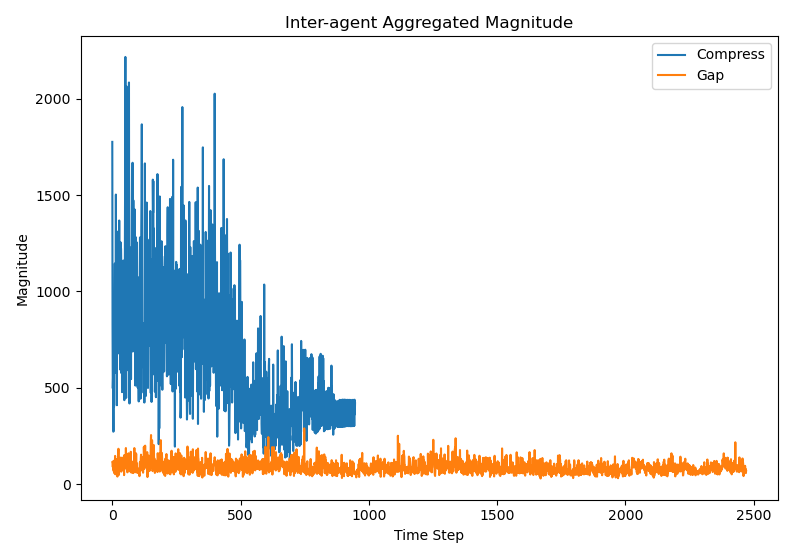
\includegraphics[width=0.8\linewidth]{figures/CompressionEffect1}
	\caption[Compression Effect]{Comparison of magnitude change using gap reduction and perimeter compression}
	\label{fig:compressioneffect1}
\end{figure}

The graph shows that the agents inter-magnitudes are effected and the swarm stablises rapidly removing internal voids (Fig.~\ref{fig:voidRemoval}). The graph shows a comparison of the new method to the existing method by Eliot et al.~\cite{eliot2019void}.

\begin{figure}
\centering
\begin{subfigure}{.4\textwidth}
	\centering	
	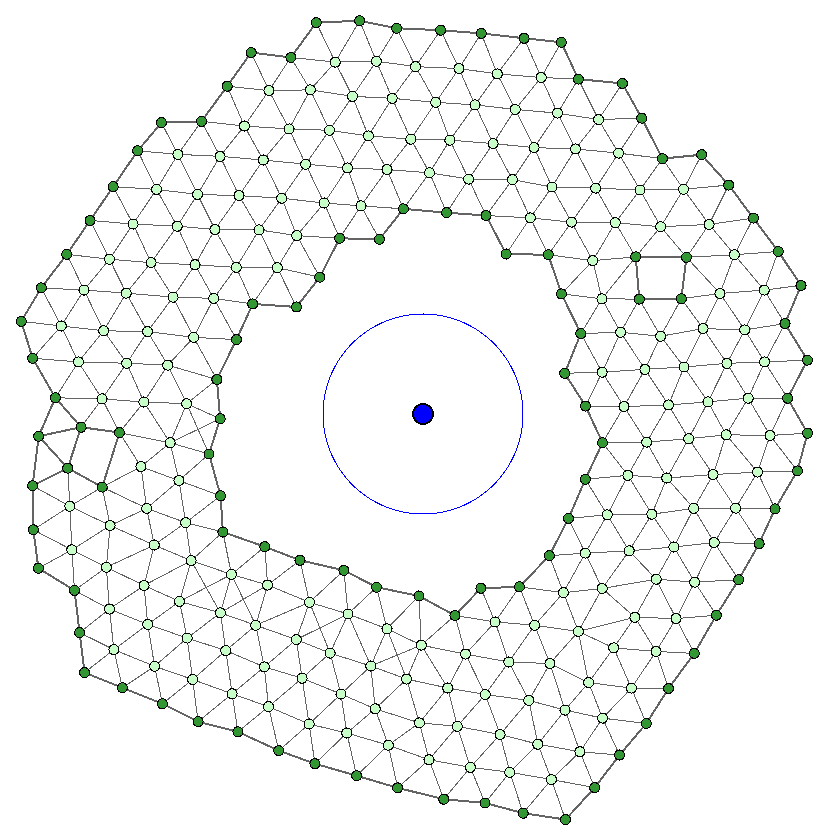
\includegraphics[width=1.0\linewidth]{figures/voidRemoval1}
	\caption[Void removal start]{Void removal start}
	\label{fig:voidRemovalStart}
\end{subfigure}
\begin{subfigure}{.4\textwidth}
	\centering
	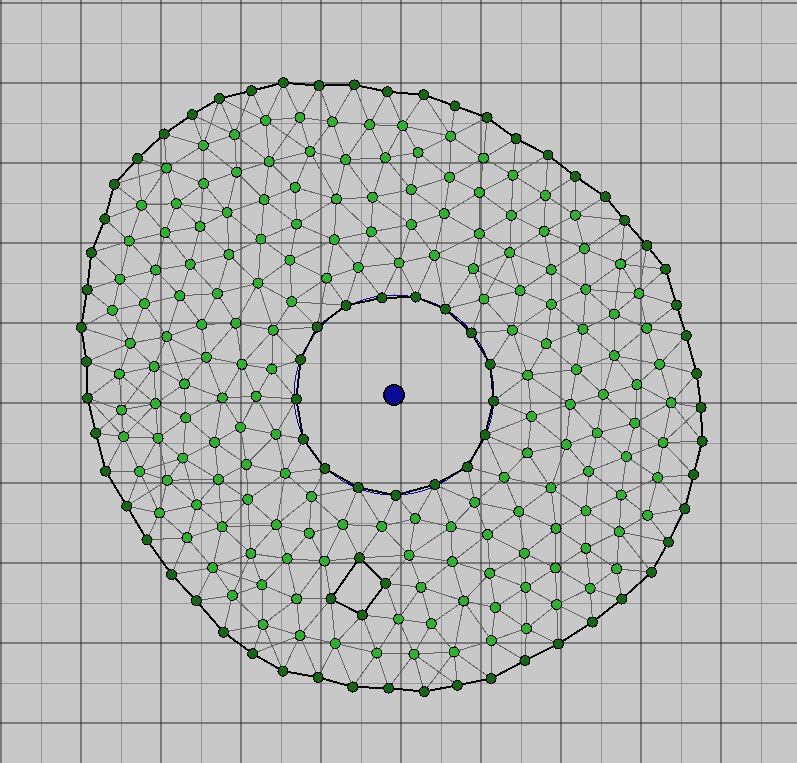
\includegraphics[width=1.0\linewidth]{figures/voidRemoval2}
	\caption[Void removal finish]{Void removal finish}
	\label{fig:voidRemovalFinish}
\end{subfigure}
\caption{Void removal through perimeter compression}
\label{fig:voidRemoval}
\end{figure}


\section{Perimeter detection}\label{perimeterDetection}
For perimeter compression to be applied to a swarm the perimeter needs to be detected. A perimeter can be defined as a continuous `surface' of agents that are not enclosed by other agents~\ref{fig:innerOuterPerimeters}. These agents may form an outer ({\color{green}green}) or inner ({\color{red}red}) boundary.

\begin{figure}[H]
	\begin{center}
		\includegraphics[width=5cm]{figures/PerimeterBots1}
	\end{center}
	\caption{{\color{green}Outer} and {\color{red}inner} swarm perimeters. \label{fig:innerOuterPerimeters}}
\end{figure}

The detection process is achieved using a cyclic analysis of the agents that surround an agent~(Fig.~\ref{fig:neighbours}). Ghrist et al. discusses a similar technique using sweep angles~\cite{ghrist2008surrounding} as does McLurkin et al~\cite{mclurkin2009}. 

\begin{figure}[H]
	\centering
	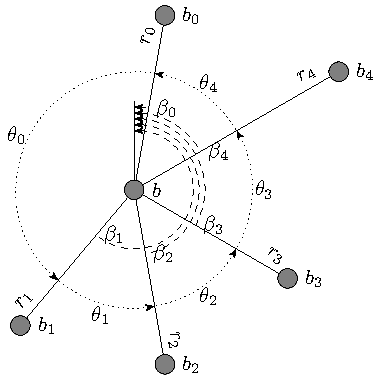
\includegraphics[width=0.8\linewidth]{figures/neighbours}
	\caption[Agent neighbours]{Agent neighbours}
	\label{fig:neighbours}
\end{figure}

The initial detection of the agents is based on the distance that each agent in the swarm is away from the current agent as described in Section~\ref{cohesion} and shown in Equation~\ref{eq:cohesion1}. The perimeter detection set is based on the range and bearing of each neighbour agent, where $r$ is the \textit{range} and $\beta$ is the \textit{bearing}~Fig.~\ref{fig:neighbours} The values are calculated  from each agent respect to $b$.

The neighbour set $N_r(b)$ is then sorted in ascending order such that $\beta_0 < \beta_1 < \ldots < \beta_n$. Each consecutive pair of agents in the sequence defines an \textit{edge}, which has length $d$ and an angle $\theta$ given by the difference in bearings of successive neighbours. The sequence of edges form a polygon that can be expressed as Equation~\ref{sortedBearing}.

\begin{equation}\label{sortedBearing}
\mathcal{P}_e = \langle (d_0,\theta_0), \ldots , (d_n,\theta_n) \rangle
\end{equation}
where
\begin{equation}
\theta_i = \beta_{i+1} - \beta_i
\end{equation}

The index addition is modulo $|\mathcal{P}_e|$, making $\beta_0$ the successor bearing to $\beta_n$ ($n+1 = 0$).  The angles $\theta$ must lie in the range $0<\theta\leq2\pi$. This restriction on the values of $\theta$ enforce the condition that

\begin{equation}
\sum\theta_i = 2\pi
\end{equation}

The length of a perimeter edge is given by the cosine rule

\begin{equation}
d_i^2 = r_{i+1}^2 + r_i^2 -2r_{i+1}r_i \cos\theta_i
\end{equation}

An agent is therefore on the perimeter of the swarm if it is not enclosed by the polygon defined in $\mathcal{P}_e$.  Simple geometry shows that this is the case, given by the predicate in Equation ~\ref{enclosing}.

\begin{equation}
\exists \theta_i \in \mathcal{P}_e : \theta_i\geq\pi
\label{enclosing}
\end{equation}

The polygon is considered to be `open' if two successive agents on the perimeter are unable to `see' one another; that is, their separation, $d$, is greater than the range of the attractive field $b_r$.  An open polygon does not enclose the agent $b$, so it is considered to be on the perimeter. 

Formally, an agent, $b$, is on the perimeter of the swarm if the predicate in Equation ~\ref{perimeter-predicate} is true.

\begin{equation}
\exists d_i\in\mathcal{P}_e:d_i>C_b \vee
\exists\theta_i\in\mathcal{P}_e:\theta_i\geq\pi
\label{perimeter-predicate}
\end{equation}

An agent is at the apex of a concave region of the perimeter if

\begin{equation}
\exists(\theta_i,d_i)\in\mathcal{P}_e : d_i>C_b\wedge\theta_i<\pi
\label{concave-predicate}
\end{equation}

The orientation is independent in so much as: if the agent $b$ is rotated through an angle of $\gamma$ then the bearings are rotated by $-\gamma$, \[ \beta_i\mapsto\beta_i-\gamma \] The  angle between successive agents is now
\footnotesize
\[
\theta_i  =  (\beta_{i+1}-\gamma) - (\beta_i-\gamma)
= \beta_{i+1}-\beta_i-\gamma+\gamma
= \beta_{i+1}-\beta_i
\]
\normalsize

\section{Repulsion compression}\label{repulsion:compression}
The repulsion compression component of the perimeter is applied by adjusted the effective range ($\mathsf{erf}(b,b')$) if the agents are both perimeter-based. Equation~\ref{eq:repulsion2} shows the new formula to calculate the adjusted repulsion. Equation~\ref{eq:repulsion2} shows the calculation of the effective field. As the agent's repulsion field is always within the cohesion field (Eq.~\ref{eq:cohesion1}), the repulsion neighbours can also be defined as a subset of the cohesion neighbours $n_c(b)$~(Eq.~\ref{eq:repulsion3}).\\

\begin{equation}\label{eq:repulsion1}
n_r(b) = \{b' \in \mathcal{S} : b \neq b' \land \lVert\vec{b b'}\rVert \leq \mathsf{erf}(b,b')\}
\end{equation}

\small
\begin{equation}\label{eq:repulsion2}
\mathsf{erf}(b, b') = \mathsf{if} \;
\mathsf{per}(b) \; \mathsf{and} \; \mathsf{per}(b') \; \mathsf{then} \;
p_rR_b \; \mathsf{else} \; R_b
\end{equation}
\normalsize


\begin{equation}\label{eq:repulsion3}
n_r(b) = \{b' \in n_c(b)~:~\magn{bb'} <= \mathsf{erf}(b,b')\}
\end{equation}

An agent is identified as a perimeter agent using the technique shown by Eliot et.al. in \cite{eliot2019void} which uses a cyclic-check of neighbour agent angles to identify ``gaps'' in the neighbours as shown in Section~\ref{perimeterDetection}.

If the condition of both agents being a perimeter is met ($\mathsf{per}(b) \; \mathsf{and} \; \mathsf{per}(b')$) the repulsion field distance is multiplied by the compression factor ($p_r$) and the new field effect is used to generate a resultant-repulsion-vector (Eq.~\ref{eq:repulsion5}). 

The effect of Equation \ref{eq:repulsion4} will be to reduce the repulsion of inter-perimeter-based agents allowing them to be closer together before a reduced repulsion-vector is applied. 

\important{The repulsion-vector that is generated is based upon $p_rR_b$, the reduced repulsion field, and not the full $R_b$ field. This is to scale the resultant-repulsion-vector as well as reducing the repulsion field.}
\small
\begin{equation}\label{eq:repulsion4}
v_r(b) = \frac{1}{\lvert n_r(b)\rvert}\sum_{b' \in n_r(b)} k_r\left(\lVert\vec{b b'}\rVert - \mathsf{erf}(b,b') \, \right)\widehat{bb'}
\end{equation}
\normalsize
\small
\begin{equation}\label{eq:repulsion5}
\mathsf{erf}(b, b') = \mathsf{if} \;
\mathsf{per}(b) \; \mathsf{and} \; \mathsf{per}(b') \; \mathsf{then} \;
p_rR_b \; \mathsf{else} \; R_b
\end{equation}
\normalsize
\section{Cohesion compression }
The cohesion component of the compression effect ($p_c$) is applied when an agent ($b$) and its neighbour ($b'$) are both perimeter-based. If the agents are not both perimeter-based then the agents vector is only scaled by $k_c$ (Eq.~\ref{eq:cohesion4}). The effect of the additional cohesion-compression weighting is to increases the size of the generated cohesion-vector $\mathsf{efc}(b,b')$ (Eq.~\ref{eq:cohesion3}). 

\begin{equation}\label{eq:cohesion3}
v_c(b) = \frac{1}{\lvert n_c(b)\rvert} \sum_{b' \in n_c(b)}\mathsf{ekc}(b, b')\, \vec{b b'}
\end{equation}

\small
\begin{equation}\label{eq:cohesion4}
\mathsf{ekc}(b, b') = \mathsf{if} \; \mathsf{per}(b) \; \mathsf{and} \; \mathsf{per}(b') \; \mathsf{then} \; \mathrm{p}_ck_c \; \mathsf{else} \; k_c
\end{equation}
\normalsize

\section{Experimental results}
For all the experiments the parameters used to create the basic swarming effect are shown in Table~\ref{tab:swarmingEffect}. The parameters create a very basic hexagonal-based distribution of agents that will stabilise as shown in Figure~\ref{fig:baselineSwarm}. The compression effect parameters are shown in Table~\ref{tab:compressionEffect} (NOTE:Probably be more than one set for the comparison - work in progress)
\begin{table}[h]
	\centering
	\tiny
	\begin{tabular}{|c|r|}
		\hline
		\rowcolor[HTML]{000000} 
		{\color[HTML]{FFFFFF} Swarming Variable} & {\color[HTML]{FFFFFF} Value} \\ \hline
		$C_b$ & \texttt{60.00} \\ \hline
		$k_c$ & \texttt{0.15}  \\ \hline
		$R_b$ & \texttt{40.00} \\ \hline
		$k_r$ & \texttt{50.00} \\ \hline
	\end{tabular}
  	\caption{Swarming effect parameters}
  	\label{tab:swarmingEffect}
\end{table}

\begin{figure}[H]
	\begin{center}
		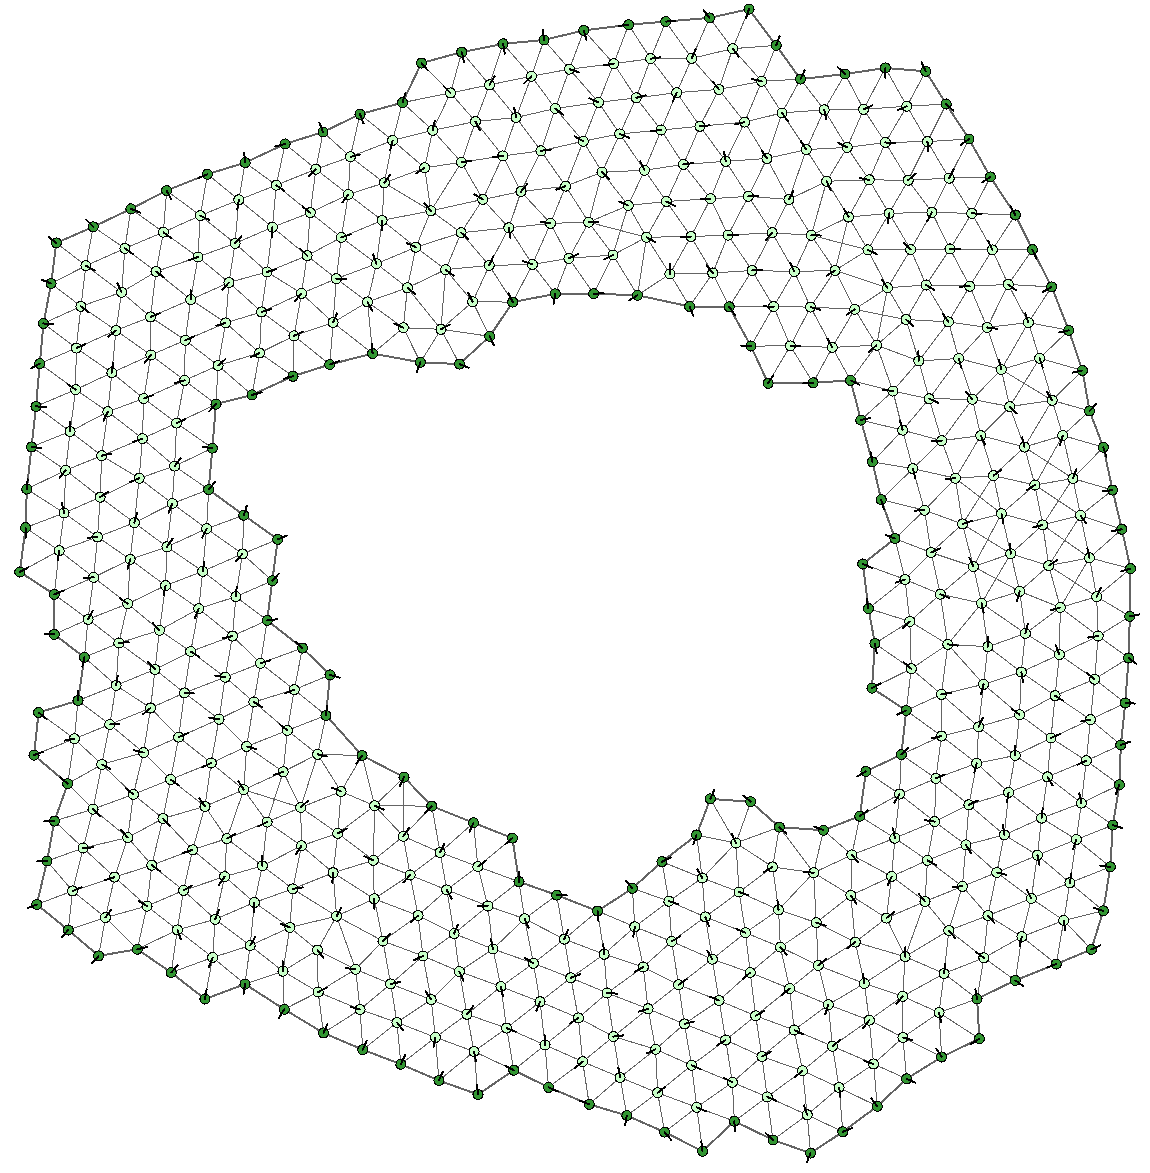
\includegraphics[width=5cm]{figures/baselineSwarm}
	\end{center}
	\caption{Baseline swarm in stablised configuration. \label{fig:baselineSwarm}}
\end{figure}

\begin{table}[h]
	\centering
	\tiny
	\begin{tabular}{|c|r|r|r|r|r|r|}
		\hline
		\rowcolor[HTML]{000000} 
		{\color[HTML]{FFFFFF} Comp.} & {\color[HTML]{FFFFFF} 1} & {\color[HTML]{FFFFFF} 2} & {\color[HTML]{FFFFFF} 3} & {\color[HTML]{FFFFFF} 4} & {\color[HTML]{FFFFFF} 5} & {\color[HTML]{FFFFFF} 6}\\ \hline
		$p_r$ & \texttt{0.10} & \texttt{0.15} & \texttt{0.20} & \texttt{0.25} & \texttt{0.30} & \texttt{0.35} \\ \hline
		$p_c$ & \texttt{20.00}  & \texttt{30.00} & \texttt{40.00} & \texttt{50.00} & \texttt{60.00} & \texttt{70.00}\\ \hline
	\end{tabular}
  	\caption{Compression effect parameters}
	\label{tab:compressionEffect}
\end{table}
\subsection{Gap compression}
\subsection{Perimeter compression}
\subsection{Comparison}

\section{Conclusions}\label{conclusions}
From the initial simulations it is possible to show that the technique is able to successfully remove voids and surround an obstacle as shown in the video \href{https://youtu.be/3eY1vvq0JWo}{https://youtu.be/3eY1vvq0JWo}.

\section{Future Work}

\bibliographystyle{abbrv}
\bibliography{perimeter}

\end{document}